\documentclass[10pt]{article}
\usepackage[a4paper,margin=1.6cm,top=1.3cm,bottom=1.3cm]{geometry}
\usepackage[T1]{fontenc}
\usepackage{lmodern}
\usepackage{microtype}
\usepackage{booktabs}
\usepackage{graphicx}
\usepackage{enumitem}
\usepackage{xcolor}
\usepackage[colorlinks=true,linkcolor=black,citecolor=black,urlcolor=blue]{hyperref}
\setlist{nosep,leftmargin=1.2em,topsep=1pt}
\setlength{\parindent}{0pt}
\setlength{\parskip}{3pt}
\pagestyle{empty}
\newcommand{\head}[1]{\par\smallskip{\large\bfseries #1}\par}
\newcommand{\sect}[1]{\par\smallskip{\bfseries\color{black!80} #1}\par}

\begin{document}
\head{Idea 2 PoC --- Do earnings streaks create disagreement?}
\textit{Proof of concept, October 2026. Code: \texttt{idea02\_streak\_disagreement/run.py}.}

\sect{Question and design}
Suppose some investors expect a streak of earnings surprises to end (gambler's fallacy) while others expect it to
continue (hot hand). Then a surprise that extends a streak should split opinions and raise trading, and Rabin and
Vayanos (2010) imply the split depends on streak length. We test this with two disagreement measures that do not
use prices. The first is \emph{abnormal turnover}: log monthly turnover minus the firm's average over the previous
year, in the announcement month and the month after. The second is the change in \emph{analyst disagreement}: the
I/B/E/S forecast standard deviation and high--low range, from the start of the announcement month to the start of
the next, scaled by price. We regress these on dummies for each signed streak length (up or down, length 2, 3, 4,
5+). Reversals, where the surprise breaks the previous sign, are the baseline. Controls are $|SUE|$, $|SUE|^2$, the
sign of the surprise, size and momentum. All regressions have month fixed effects, with SEs clustered by month. The
sample has 97{,}150 announcements, 2005--2020, with SRW surprises and streaks as in the gambler's-fallacy paper.

\begin{center}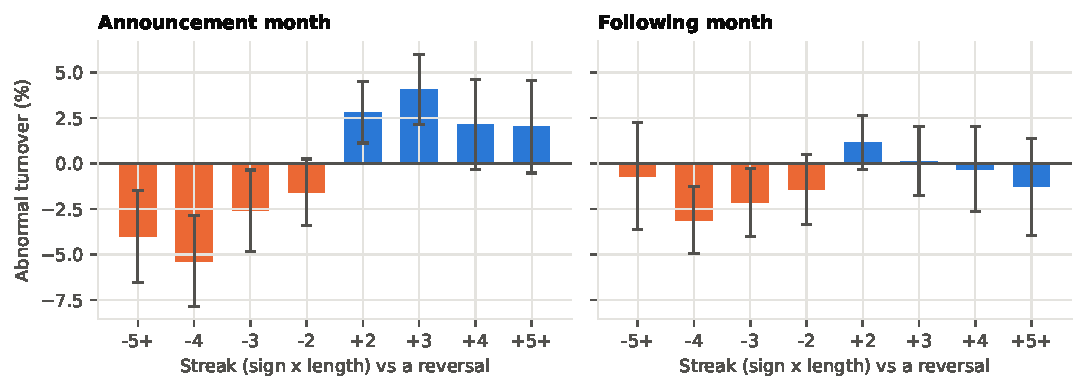
\includegraphics[width=0.97\textwidth]{results/fig_main.pdf}\end{center}

\begin{center}\small
\begin{tabular}{lcccc|cccc}
\toprule
 & \multicolumn{4}{c|}{Up-streak of length} & \multicolumn{4}{c}{Down-streak of length}\\
 & 2 & 3 & 4 & 5+ & 2 & 3 & 4 & 5+\\
\midrule
Abnormal turnover, announcement month (\%) & 2.8 & 4.1 & 2.1 & 2.0 & $-1.6$ & $-2.6$ & $-5.4$ & $-4.0$\\
 & (3.3) & (4.2) & (1.7) & (1.6) & ($-1.7$) & ($-2.3$) & ($-4.2$) & ($-3.1$)\\
Analyst range, change (bp of price) & 0.9 & 3.2 & 2.3 & 2.0 & 0.3 & $-1.0$ & $-4.9$ & $-5.5$\\
 & (1.0) & (2.7) & (1.9) & (1.9) & (0.3) & ($-0.5$) & ($-1.8$) & ($-2.3$)\\
\bottomrule
\end{tabular}\\[2pt]
{\footnotesize Differences relative to a reversal of the same sign ($t$-statistics). The analyst SD shows no
significant pattern. Drift test: the streak drift is not stronger in high-turnover announcements (SUE $\times$
continuation $\times$ high turnover $=0.13$, $t=0.95$).}
\end{center}

\sect{Findings}
\begin{itemize}
\item \textbf{Streaks change trading, but the effect depends on the sign.} Good-news streaks raise turnover, most at
  length 3 (+4.1\%), and analyst forecasts spread out (+3.2 bp). Bad-news streaks lower turnover, more the longer
  they get ($-5.4\%$ at length 4), and analyst forecasts converge ($-5.5$ bp at 5+).
\item \textbf{This is only partly the predicted disagreement.} Rising disagreement fits good-news streaks, but a
  long bad-news streak \emph{reduces} disagreement and trading. A plausible alternative is the disposition effect:
  holders of stocks with good-news streaks sit on gains and sell into the news, while holders of stocks with
  bad-news streaks sit on losses and hold. Momentum is controlled for, but capital-gains overhang is not.
\item \textbf{Disagreement does not explain the price drift.} The streak drift is no stronger in high-turnover
  announcements.
\end{itemize}

\sect{Assessment and next steps}
A robust new fact (volume is asymmetric in streak sign and length), but the disagreement interpretation is not
established. To make it a paper: (i) add the capital-gains overhang from Idea 10 as a control or competing
explanation; (ii) use daily volume and order-imbalance data to separate buying from selling; (iii) use
analyst-level detail data to measure true dispersion. As it stands, the evidence is better suited to a
mechanism section of the gambler's-fallacy paper than to a standalone Q1 paper.
\end{document}
